\documentclass[12pt]{scrartcl}

\usepackage{amsthm}
\usepackage{amsmath}
\usepackage{graphicx}
\usepackage{fancyvrb}


\title{Lecture Notes week 3}
\author{\"Omer \c Sakar}
\date{\today}

\newtheorem{defi}{Definition}
\newtheorem{theo}{Theorem}



\begin{document}
\maketitle
\tableofcontents
\newpage

\section{Lecture 1}
$k^{-\gamma - 1}\ or\ k^{-\tau},\ with\ \tau = \gamma + 1\ and\ \gamma \in (1,3)$\\
$P_{k} \approx const\cdot k^{-\gamma - 1}$\\
$\bar{F}_{k} = P(x \geq k) = \sum\limits_{s=k}^\infty P_{s} \approx c\cdot k^{-\gamma}$



\begin{figure}[h]
	\centering
	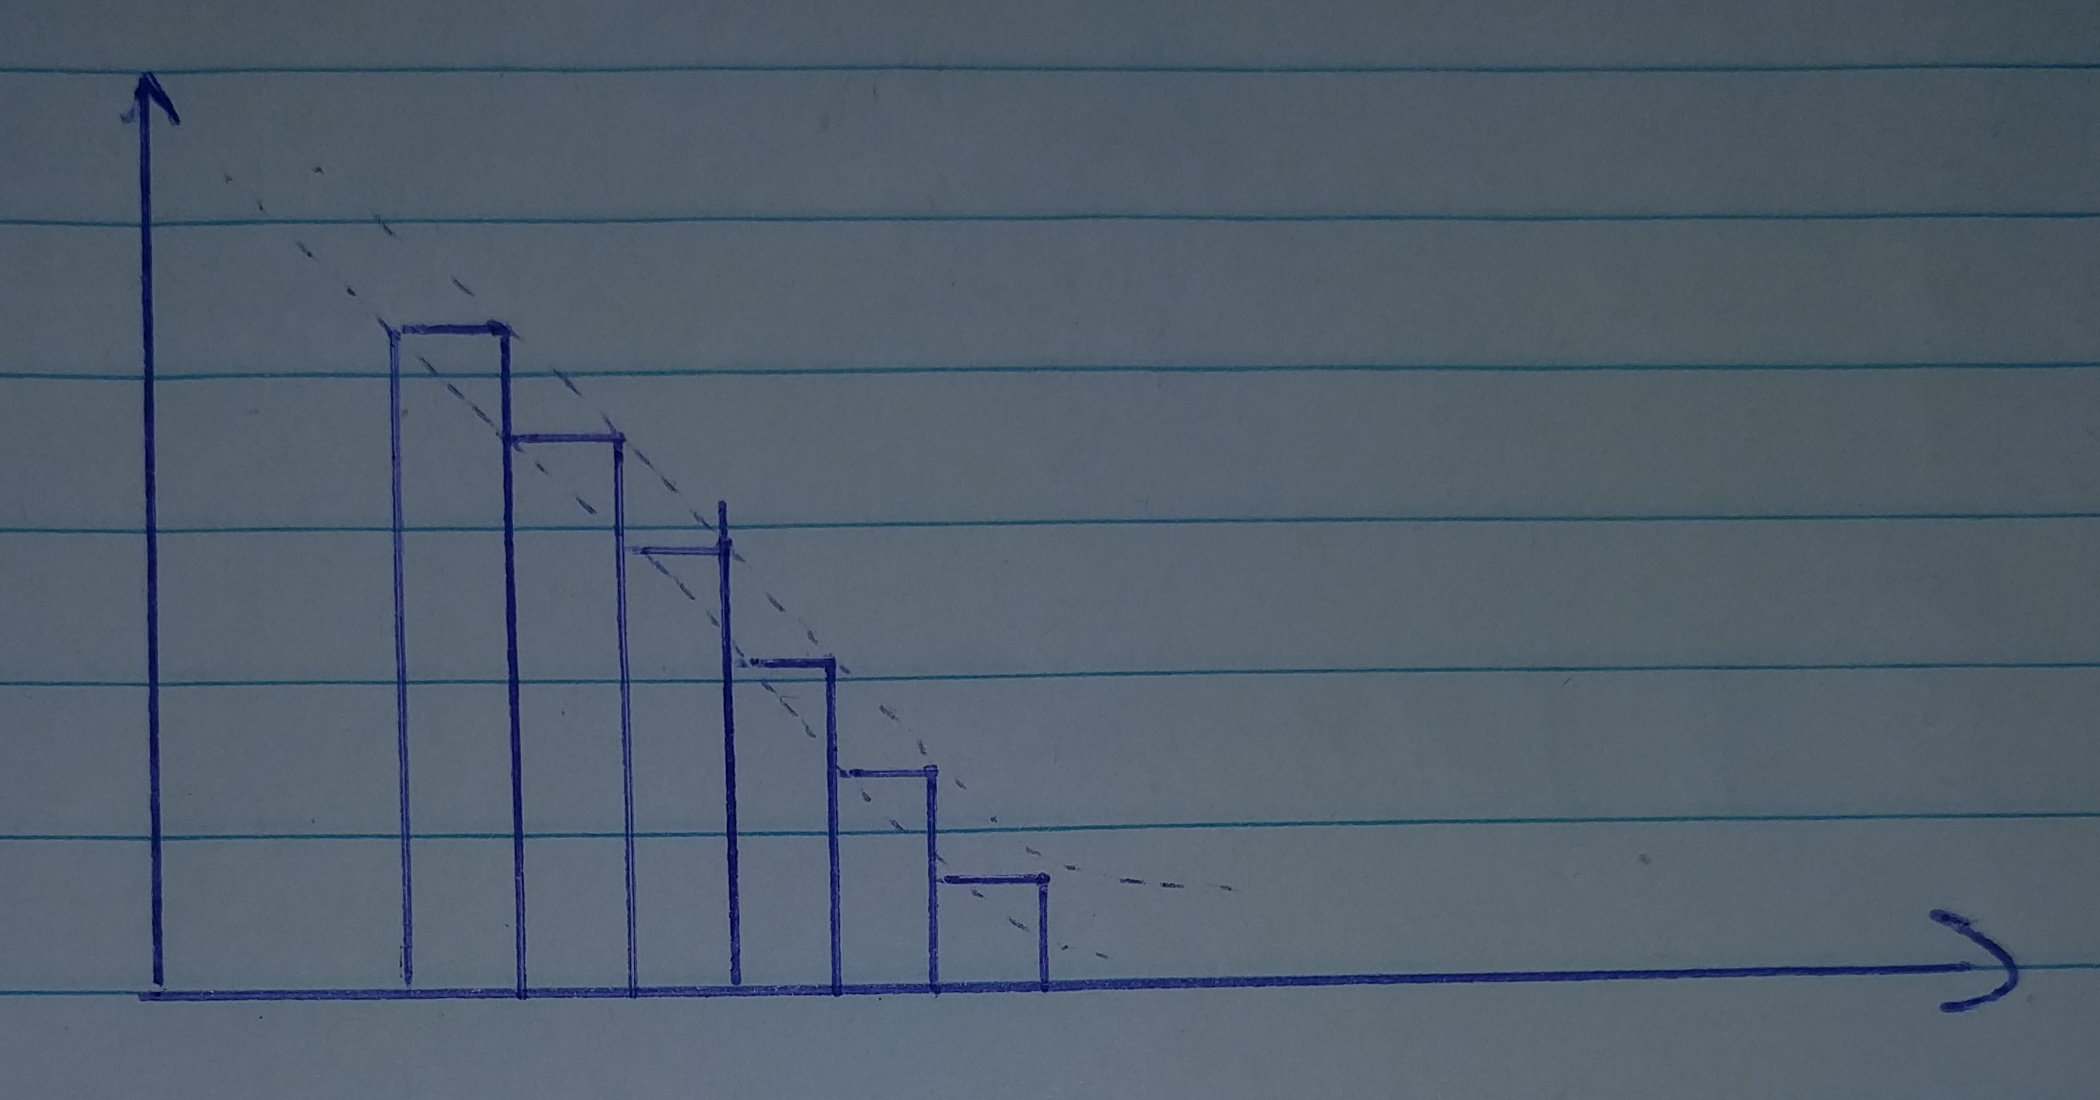
\includegraphics[width=\textwidth]{./images/fig_1.jpg}
	\captionof{figure}{Visual representation of the formula on slide 4.}    
\end{figure}

\noindent $EX^{2} = \sum\limits_{k=k_{0}}^\infty k^{2}\cdot c\cdot k^{-\gamma-1} = \sum\limits_{k=k_{0}}^\infty c\cdot k^{1 - \gamma} < \infty \iff \gamma > 2$\\



\noindent $X_{1},X_{2},X_{3}\dotsc \dotsc$ - Independent and identically distributed random variable.\\
LLN: $\frac{X_{1} + X_{2} + \dotsc \dotsc X_{n}}{n} \stackrel{\rightarrow}{a.s.} EX\ (the\ mean)$\\
\indent \indent$\ \ \sum\limits_{i=1}^n X_{i}^{P} \approx n^{\frac{P}{j}}$



\subsection{Preferential Attachment (PA)}
A new node connects to an existing node with probability proportional to the degree of the existing node, (the idea of of "the rich get richer").
The degree of a new node $m$, we coinsider $m=1$.

New node connects to an existing node with probability proportional to the degree $m = \#$ of links of a new node.
\begin{defi}
	$P_{k,t}$ is the fraction of nodes with degree $k$ at time 	$t$ (after node $t$ arrived).
\end{defi}

$\sum\limits_{k=m}^\infty k\cdot P_{k,t} = \frac{1}{t}\cdot \sum\limits_{k=m}^\infty k\cdot [\#\ of\ nodes\ with\ degree\ k] = \frac{1}{t}\cdot [total\ degree] = \frac{2\cdot m\cdot t}{t} = 2\cdot m$\\

\noindent The probability that a new node connects to a new node with degree k is:\\

$\frac{k\cdot [\#\ of\ nodes\ with\ degree\ k]}{\sum\limits_{l=m}^\infty l\cdot [\#\ of\ nodes\ with\ degree\ k]} \stackrel{(divide\ by\ t)}{=} \frac{k\cdot P_{k,t}}{\sum\limits_{l=m}^\infty l\cdot P_{k,t}} = \frac{k\cdot P_{k,t}}{2\cdot m}$\\

\noindent Change in number of nodes with degree $k$ at $t+1$:

$(t+1)\cdot P_{k,t+1} - t\cdot P_{k,t} = \frac{(k-1)\cdot P_{k-1,t}}{2\cdot m}\cdot m - \frac{k\cdot P_{k,t}}{2\cdot m}\cdot m,\ with\ k>m$

$(t+1)\cdot P_{m,t+1} - t\cdot P_{m,t} = 1 - \frac{m\cdot P_{m,t}}{2\cdot m}\cdot m$\\

\noindent The questions we have to solve are:

Solve for $t \rightarrow \infty$

$P_{k} = \frac{1}{2}\cdot (k-1)\cdot P_{k-1} - \frac{1}{2}\cdot k\cdot P_{k},\ with\ k>m$\\
\indent $P_{m} = 1 - \frac{1}{2}\cdot m\cdot P_{m}$\\


\noindent Solutions:

\indent $P_{m}\cdot (\frac{1}{2} m + 1) = 1 \implies P_{m} = \frac{2}{m + 2}$

\indent $P_{k} = \frac{(k-1)(k-2)(k-3)\dotsc \dotsc \cdot m}{(k+2)(k+1)\dotsc \dotsc \cdot m +3} = \frac{2\cdot m\cdot (m+1)}{
k\cdot (k+1)\cdot (k+2)
}
\approx c\cdot k^{-3}$\newline

\noindent Zipf's Law is for self-study.

\subsection{Maximal degree}
$D_{1},D_{2},D_{3},\dotsc \dotsc D_{n}$ - Degrees\\
$P(D>x) \approx c\cdot x^{-\gamma}$\\
Maximal degree $\implies$ Largest value $\implies$ probability is $\frac{1}{n}$\\
$P(D>d_{max}) \approx \frac{1}{n} \approx c\cdot (d_{max})^{-\gamma}$\\
$d_{max} = c'\cdot n^{\frac{1}{\gamma}}$\\

\noindent $j$-th largest value $d^{(j)}$\\
$P(D>d^{(j)}) \approx \frac{j}{n} \approx c\cdot (d^{(j)})^{-\gamma}$\\
$d^{(j)} \approx c"\cdot n^{\frac{1}{\gamma}}\cdot j^{-\frac{1}{\gamma}}$

\begin{figure}[h]
	\centering
	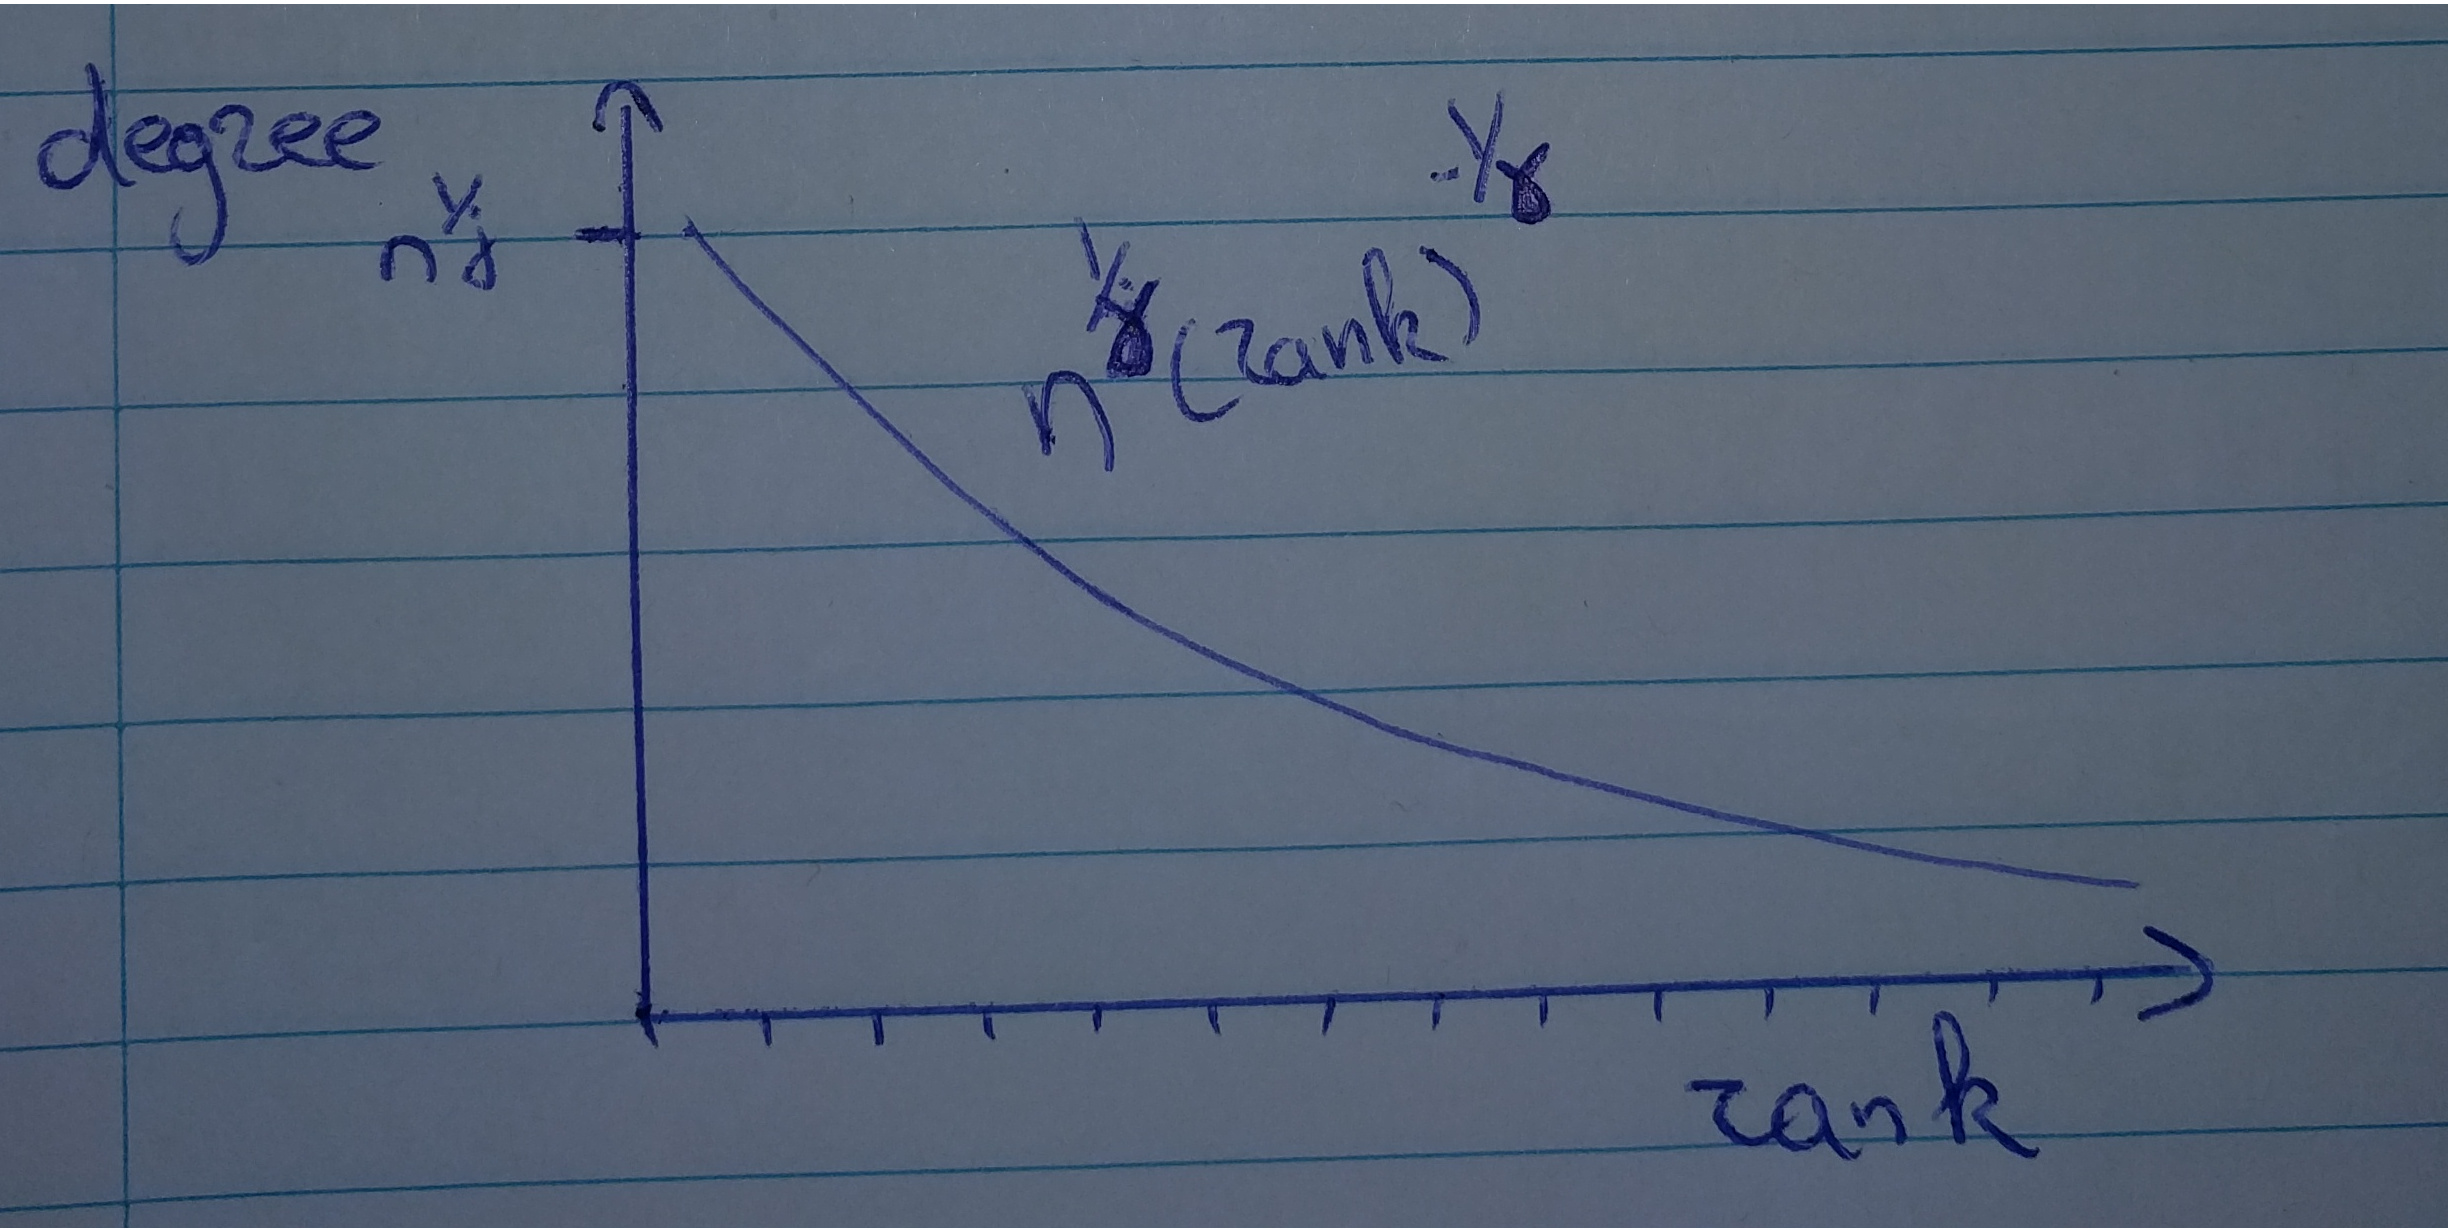
\includegraphics[width=\textwidth]{./images/fig_2.jpg}
	\captionof{figure}{Nice picture with text.}    
\end{figure}


\clearpage
\section{Lecture 2 Innovation diffusion through a network} 

\begin{figure}[h]
	\centering
	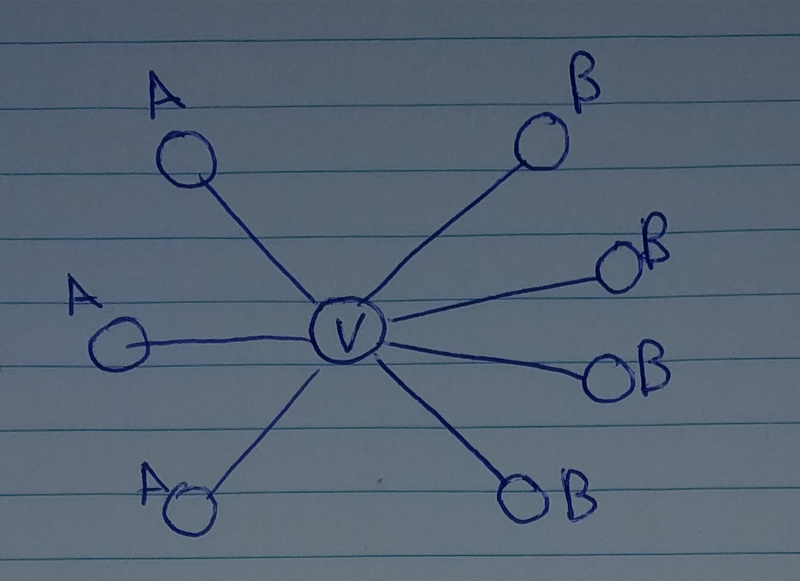
\includegraphics[width=0.5\textwidth]{./images/fig1.jpg}
 
\end{figure}

\begin{figure}[h]
	\centering
	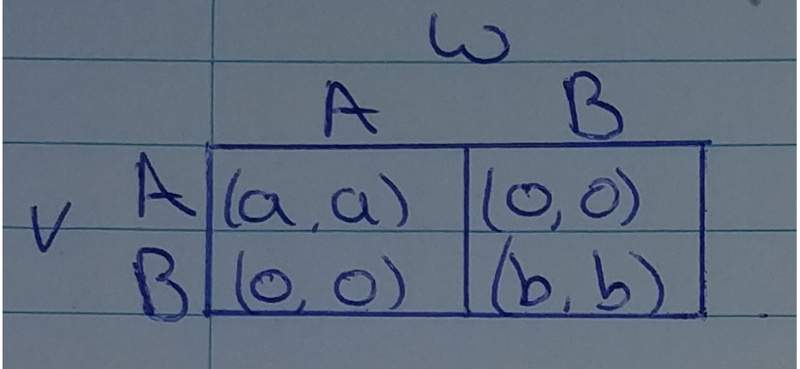
\includegraphics[width=0.5\textwidth]{./images/fig2.jpg}
  
\end{figure}

\begin{defi}
	Fraction p of the neighbours of v adapted A.\\
	Fraction 1-p of the neighbours of v adapted B.
\end{defi}

Adapting A: reward dpa\\
Adapting B: reqard d(1-p)b\\


Adapt A if $dpa > d(1-p)b \implies pa > (1-p)b \implies p(a+b) > b$

We can rewrite this as (this is important):
\begin{itemize}
\item $p > \frac{b}{a+b} \implies$ adapt A
\item $p < \frac{b}{a+b} \implies$ adapt B
\item $p = \frac{b}{a+b} \implies$ adapt A (This is something we decided)
\end{itemize}

\noindent Example: if $a = b \implies \frac{b}{a+b} = \frac{1}{2}$.
  
\begin{itemize}
\item Step 0: all B
\item Step 1: $u \rightarrow A$, $v \rightarrow A$
\item Step 2: $x \rightarrow A$
\item Step 3: $y \rightarrow A$, $w \rightarrow A$
\item Step 4: $z \rightarrow A$
\end{itemize}

\begin{figure}[h]
	\centering
	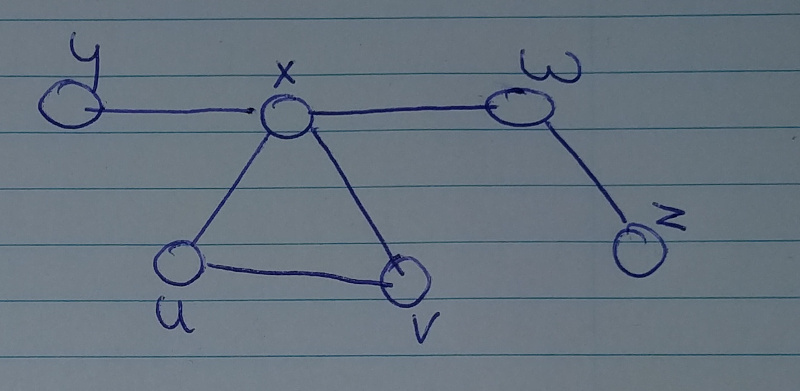
\includegraphics[width=0.5\textwidth]{./images/fig3.jpg}
\end{figure}

The result is a cascade which results in the whole network being A.

If we were to add a node a to the neighbourhood of x, the cascading effect stops.\\


Example Clusters
\begin{defi}
	Cluster of density 1-q is a set of nodes, each of which has at least 1-q fraction of their links in the cluster.
\end{defi}

\begin{figure}[h]
	\centering
	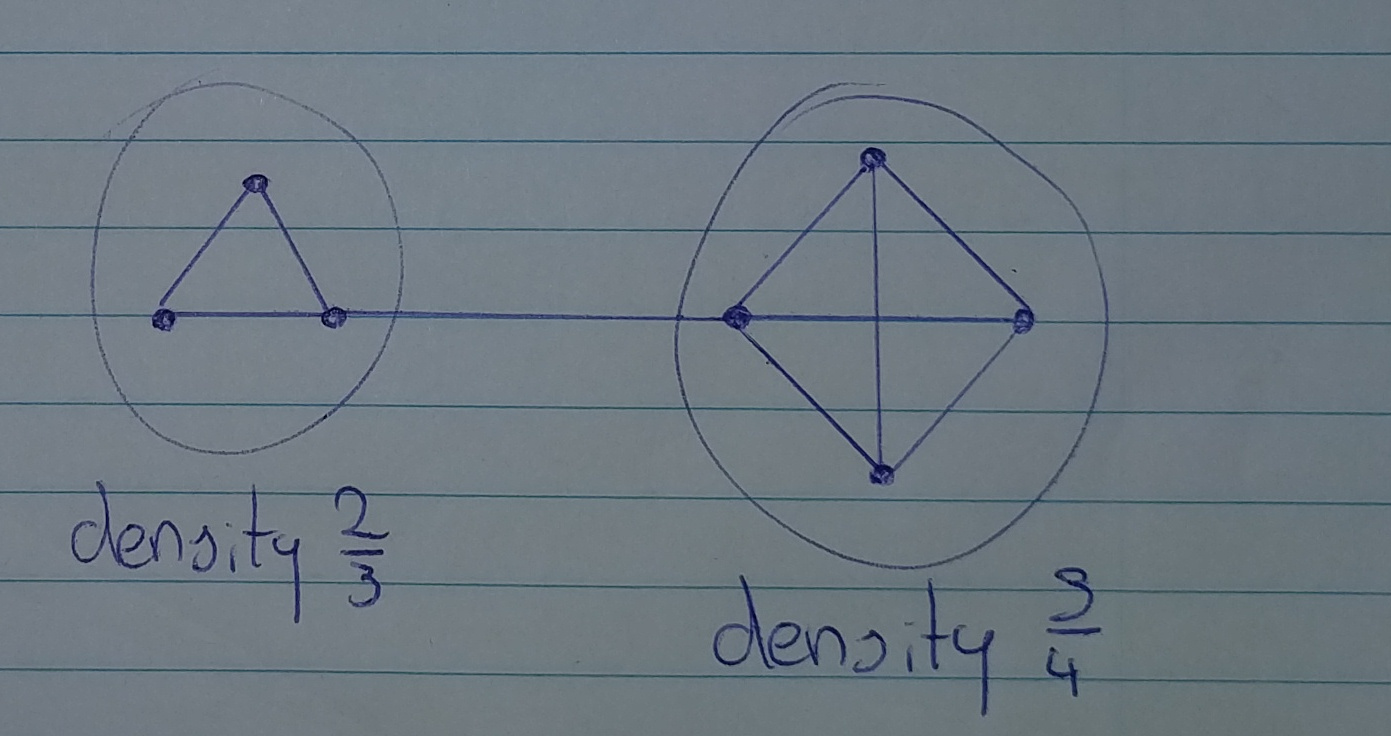
\includegraphics[width=0.7\textwidth]{./images/fig4.jpg}
\end{figure}

Claim: Denote $q = \frac{b}{a+b}$. Consider a set of inital adapters of A. The cascade is not complete $\iff$ network contains a cluster of density $> 1-q$ (without the initial adapters).

Cascading behaviour: $[fraction \geq q]$ adapted A $\implies$ the node adapts A.

\begin{figure}[h]
	\centering
	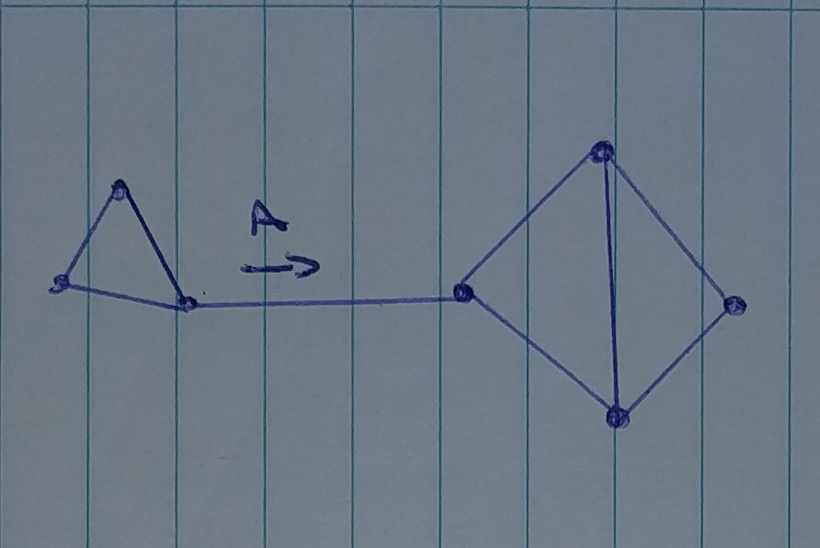
\includegraphics[width=0.7\textwidth]{./images/fig5.jpg}
	\caption{For this to happen, $q\leq \frac{1}{3}$. Think about $q$ as a threshold. The lower the threshold, the easier to go over it}
\end{figure}
\clearpage

Example Hubs:


\begin{figure}[h]
	\centering
	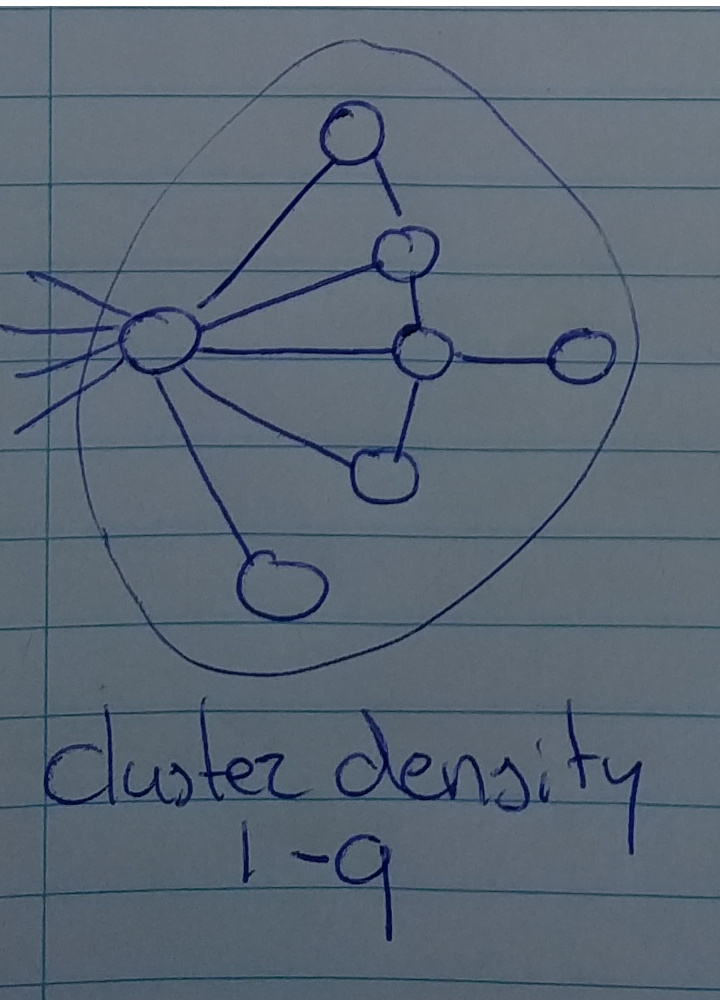
\includegraphics[width=0.3\textwidth]{./images/fig6.jpg}
\end{figure}


\subsection{Knowledge and collective action (chapter 19.6)}
I act only if at least k peiple act. I know only what my neighbours do. Solution: common knowledge.\\

How to choose inital adapters? Influence maximization 2003
Competitive technologies. (dont know what is means, but they are in my notes, so I kept them in)\\

\subsection{Small World Phenomenon SWP}
$U_{1}, U_{2}$ - 2 random nodes.\\
$d(U_{1}, U_{2})$ - graph distance between $U_{1}$ and $U_{2}$.\\
$d(U_{1}, U_{2}) < \infty$ (the path exists).\\

\noindent The SWP states $d(U_{1}, U_{2}) = O(log n)$ with n = number of nodes. Let $h_{n} = d(U_{1}, U_{2})$
$\exists\ c>0, P(H_{n} > c\cdot log(n)) = O(1),\ n\rightarrow \infty$.\\

\noindent Explanation: regular tree with number of offspring d.
\begin{figure}[h]
	\centering
	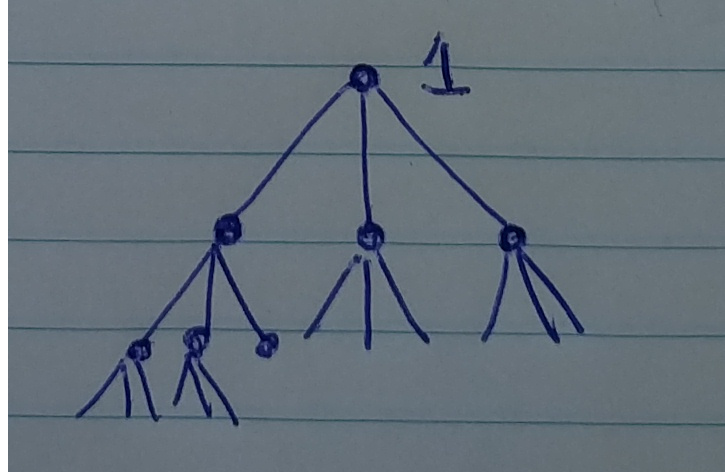
\includegraphics[width=0.35\textwidth]{./images/fig7.jpg} 
\end{figure}


\noindent Number of nodes at distance 1: $d$\\
Number of nodes at distance 2: $d^{2}$\\
\vdots						 \\
Number of nodes at distance k: $d^{k} \leftarrow last generation$\\

\noindent $1 + d + d^{2} + \cdots + d^{k} = n$\\
$\frac{d^{k+1}-1}{d-1} \approx c\cdot d^{k} = n$ where $k = log(n) - c$

















\end{document}